% Tree (tomato plant) experiment — results.
% Companion to tree_experiment_setup.tex; requires booktabs and siunitx.
% GradientNBV numbers are final (4/4 orientations valid at every level).
% RH-NBV cells marked \todo are pending the reach-clamped reruns
% (blossom x4, whole-plant y090/y180); fill from analyze_tree_results.py,
% then bold the better value per row (higher = better for quality metrics,
% lower = better for view counts and path length).

\section{Plant Experiment: Results}

\subsection{Fruit level}
\label{sec:tree-results-fruit}

Table~\ref{tab:tree-fruit-results} summarises the fruit-level reconstruction
over the four plant orientations, and
Figure~\ref{fig:tree-fruit-curves} shows the per-view progression.

\begin{table}[t]
\centering
\begin{tabular}{lcc}
\toprule
 & GradientNBV & RH-NBV \\
\midrule
\multicolumn{3}{l}{\itshape Reconstruction quality after 20 views} \\
\quad ROI coverage (\%)     & $92.9 \pm 2.8$    & $\mathbf{97.3 \pm 1.4}$ \\
\quad $F_1$ score           & $0.961 \pm 0.014$ & $\mathbf{0.990 \pm 0.007}$ \\
\quad Recall                & $0.925 \pm 0.026$ & $\mathbf{0.980 \pm 0.013}$ \\
\addlinespace
\multicolumn{3}{l}{\itshape Convergence speed} \\
\quad Views until \SI{80}{\percent} coverage & $\mathbf{4.2 \pm 0.4}$ & $4.5 \pm 0.5$ \\
\quad Views until \SI{90}{\percent} coverage & $10.7 \pm 3.1$\,$^{a}$ & $\mathbf{8.5 \pm 2.2}$ \\
\addlinespace
\multicolumn{3}{l}{\itshape Motion cost} \\
\quad End-effector path length (m) & $\mathbf{0.44 \pm 0.12}$ & $2.50 \pm 0.62$ \\
\bottomrule
\end{tabular}
\caption{Fruit-level results on the tomato plant under natural occlusion;
mean $\pm$ standard deviation over the four plant orientations (20 views per
run). Bold marks the better value in each row: higher is better for the
quality metrics, lower is better for the view counts and the path length.
Coverage is the fraction of ground-truth fruit
surface points observed at least once; $F_1$ and recall compare the
reconstructed voxel centres against the ground-truth fruit surface at the
\SI{6}{\milli\metre} matching threshold of Section~\ref{sec:tree-setup}.
$^{a}$\,GradientNBV failed to reach \SI{90}{\percent} coverage within the
20-view budget at one orientation; its mean is computed over the remaining
three.}
\label{tab:tree-fruit-results}
\end{table}

\begin{figure}[t]
\centering
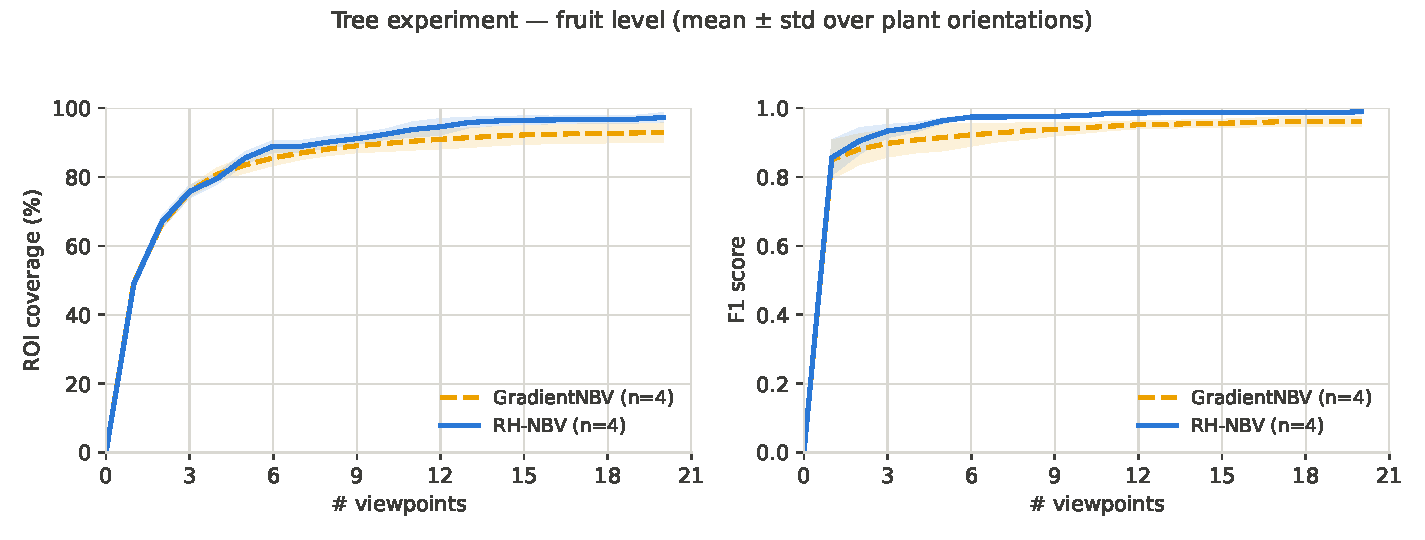
\includegraphics[width=\linewidth]{figures/tree/fruit_curves.pdf}
\caption{Fruit-level ROI coverage (left) and $F_1$ (right) per viewpoint,
mean $\pm$ one standard deviation over the four plant orientations.}
\label{fig:tree-fruit-curves}
\end{figure}

Three observations stand out. First, during the initial viewpoints the two
planners are equivalent: both reach \SI{80}{\percent} ROI coverage after
$4$--$5$ views, since the freely visible portion of the fruit cluster can be
captured by any reasonable strategy. The advantage of receding-horizon
planning only materialises where occlusion dominates. GradientNBV plateaus at
\SIrange{90}{93}{\percent} coverage at every orientation -- its local
gradient steps keep the camera near already-observed surfaces and cannot
recover fruit regions hidden behind foliage -- and at one orientation it
never reaches the \SI{90}{\percent} threshold within the 20-view budget.
RH-NBV continues to convert occluded fruit surfaces throughout the run and
attains \SIrange{95}{98}{\percent} coverage at all four orientations,
reaching \SI{90}{\percent} coverage $2.2$ views earlier on average.\\

Second, RH-NBV is not only better on average but also more consistent: its
standard deviation is smaller for every accuracy metric (e.g.\ $\pm 1.4$ vs.\
$\pm 2.8$ percentage points of final coverage), even though the four
orientations expose the planners to visibly different occlusion patterns
(first-view fruit recall ranges from $0.72$ to $0.88$). The receding-horizon
search compensates for unfavourable orientations that trap the purely local
baseline.\\

Third, the accuracy gain is paid for in motion: RH-NBV travels roughly six
times the end-effector path length ($2.50$ vs.\ \SI{0.44}{\metre} on
average). In applications where cycle time or energy dominates, this
trade-off must be weighed; where perception completeness of occluded fruit
is the objective -- as in harvesting -- the additional motion buys the
decisive difference between a plateaued and a near-complete reconstruction.
No planner hyper-parameters were retuned for the plant scenes
(Section~\ref{sec:tree-setup}), so these results also indicate that the proposed
planner generalises across object classes without adjustment.

\subsection{Blossom level}
\label{sec:tree-results-blossom}

% TODO(RH rerun): fill the RH-NBV column from analyze_tree_results.py once the
% reach-clamped blossom runs (4 orientations) finish; then bold per row and
% write the discussion. Gradient column below is FINAL.
Table~\ref{tab:tree-blossom-results} summarises the blossom-level
reconstruction over the four plant orientations.

\begin{table}[t]
\centering
\begin{tabular}{lcc}
\toprule
 & GradientNBV & RH-NBV \\
\midrule
\multicolumn{3}{l}{\itshape Reconstruction quality after 20 views} \\
\quad ROI coverage (\%)     & $97.6 \pm 0.2$    & --- \\
\quad $F_1$ score           & $0.932 \pm 0.040$ & --- \\
\quad Recall                & $0.877 \pm 0.067$ & --- \\
\addlinespace
\multicolumn{3}{l}{\itshape Convergence speed} \\
\quad Views until \SI{80}{\percent} coverage & $4.0 \pm 0.0$ & --- \\
\quad Views until \SI{90}{\percent} coverage & $7.5 \pm 1.1$ & --- \\
\addlinespace
\multicolumn{3}{l}{\itshape Motion cost} \\
\quad End-effector path length (m) & $0.47 \pm 0.04$ & --- \\
\bottomrule
\end{tabular}
\caption{Blossom-level results on the tomato plant under natural occlusion;
mean $\pm$ standard deviation over the four plant orientations (20 views per
run). Bold marks the better value in each row: higher is better for the
quality metrics, lower is better for the view counts and the path length.
Coverage is the fraction of ground-truth blossom surface points observed at
least once; $F_1$ and recall use the \SI{8}{\milli\metre} matching threshold
of Section~\ref{sec:tree-setup}.}
\label{tab:tree-blossom-results}
\end{table}

% TODO: 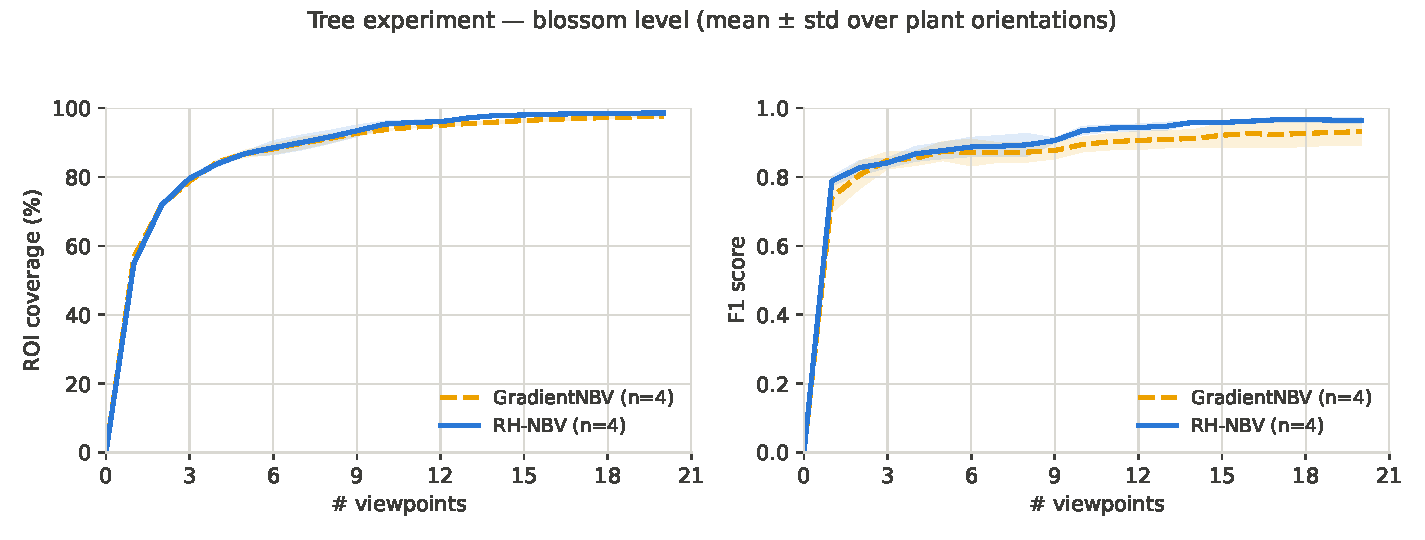
\includegraphics{figures/tree/blossom_curves.pdf} once generated.

\subsection{Whole-plant level}
\label{sec:tree-results-all}

% TODO(RH rerun): RH-NBV column pending reach-clamped y090/y180 makeups; the
% two currently valid orientations (y000, y270) give cov 91.2+-2.5,
% F1 0.922+-0.042, traj 1.35+-0.57 — preliminary trend: GradientNBV LEADS at
% this level (whole plant is mostly self-visible, so exploration pays less
% and costs more motion). Report honestly; note y270 precision anomaly (0.79)
% under investigation. Gradient column below is FINAL.
Table~\ref{tab:tree-all-results} summarises the whole-plant reconstruction
over the four plant orientations.

\begin{table}[t]
\centering
\begin{tabular}{lcc}
\toprule
 & GradientNBV & RH-NBV \\
\midrule
\multicolumn{3}{l}{\itshape Reconstruction quality after 20 views} \\
\quad ROI coverage (\%)     & $96.6 \pm 0.8$    & --- \\
\quad $F_1$ score           & $0.992 \pm 0.002$ & --- \\
\quad Recall                & $0.984 \pm 0.004$ & --- \\
\addlinespace
\multicolumn{3}{l}{\itshape Convergence speed} \\
\quad Views until \SI{80}{\percent} coverage & $4.0 \pm 0.0$ & --- \\
\quad Views until \SI{90}{\percent} coverage & $8.8 \pm 0.8$ & --- \\
\addlinespace
\multicolumn{3}{l}{\itshape Motion cost} \\
\quad End-effector path length (m) & $0.55 \pm 0.03$ & --- \\
\bottomrule
\end{tabular}
\caption{Whole-plant results on the tomato plant; mean $\pm$ standard
deviation over the four plant orientations (20 views per run). Bold marks the
better value in each row: higher is better for the quality metrics, lower is
better for the view counts and the path length. Coverage is the fraction of
ground-truth plant surface points observed at least once; $F_1$ and recall
use the \SI{10}{\milli\metre} matching threshold of
Section~\ref{sec:tree-setup}.}
\label{tab:tree-all-results}
\end{table}

% TODO: 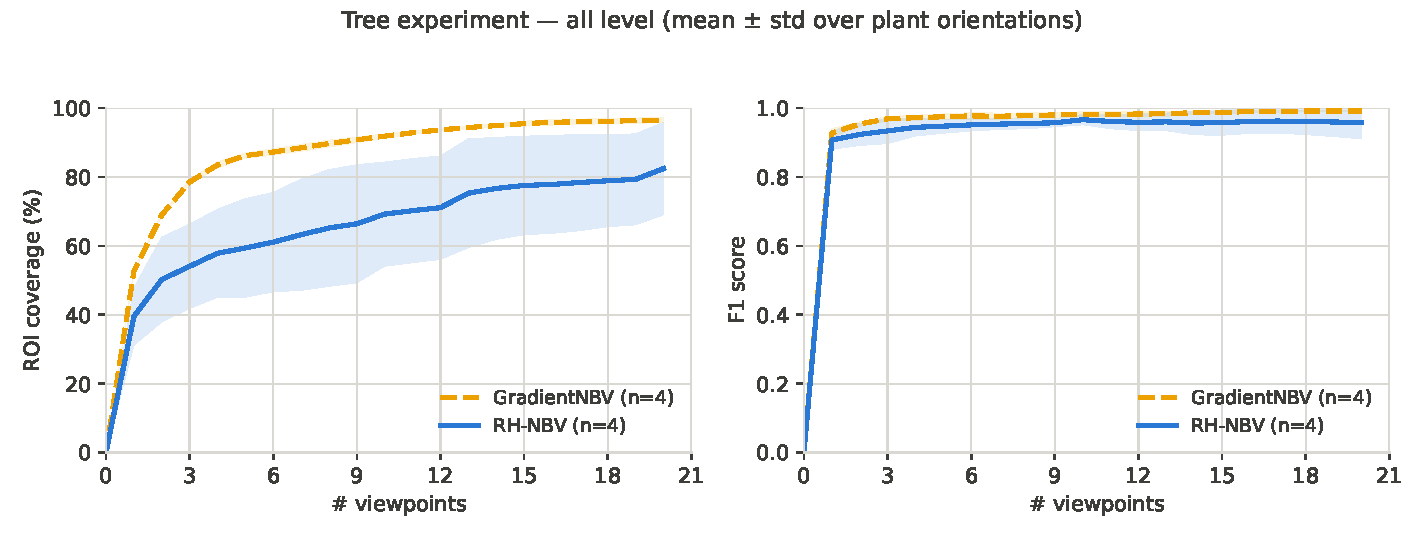
\includegraphics{figures/tree/all_curves.pdf} once generated.
